\documentclass[a4paper,10pt]{article}

\usepackage{tabularx}
\usepackage{graphicx}
\usepackage{geometry}
\geometry{
    top=2cm,
    bottom=2cm,
    left=1cm,
    right=1cm
}

\usepackage{xepersian}
\settextfont{Vazirmatn-Regular.ttf}

\title{TOMSAC - روش مدیریت تعادل بین ایمنی خودرویی و امنیت سایبری}
\author{}
\date{}

\linespread{1.5}

\begin{document}

    \maketitle

    \begin{abstract}
        
        وابستگی‌های متقابل ایمنی و امنیت برای محققان چندین دهه مورد توجه بوده است. با این حال، در عمل، به دلایل مختلفی از جمله عدم درک کافی و تمایل به تغییر رویه‌های فعلی، توجه لازم به آن‌ها نمی‌شود. این تحقیق با هدف پیشبرد وضعیت هنر در این زمینه با توسعه یک روش عملی، آسان برای انطباق و استفاده برای مدیریت وابستگی‌ها و تعادل‌ها در طول دوره توسعه سیستم‌های سایبر-فیزیکی انجام شده است. این روش به نام TOMSAC که مخفف مدیریت تعادل بین ایمنی و امنیت سایبری است، نامیده شده است.

    \end{abstract}

    \section{مقدمه}

        یک بررسی جامع از روش‌های مهندسی مشترک برای ایمنی و امنیت سایبری در سراسر حوزه سایبر-فیزیکی توسط Kavallieratos و همکاران (2020) ارائه شده است. این مقاله یک بررسی جامع از 68 روش مهندسی مشترک ایمنی و امنیت سایبری ارائه می‌دهد و به مسائل باز و چالش‌های پژوهشی مرتبط می‌پردازد. این 68 روش به دو دسته "یکپارچه" (یعنی دو فرآیند جداگانه مرتبط ایمنی و امنیت) و "ترکیبی" (یعنی یک فرآیند یکپارچه که هم ایمنی و هم امنیت را ترکیب می‌کند) تقسیم می‌شوند. 37 روش از روش‌های بررسی‌شده یکپارچه هستند و 31 روش ترکیبی. بیشتر روش‌های بررسی‌شده مدل‌محور هستند (52 از 68) و برای یک حوزه کاربردی واحد توسعه یافته‌اند (45). تنها 20 روش با استانداردهای مربوطه اطلاعاتی دارند و جالب این است که اکثر روش‌های بررسی‌شده (49) به مسئله حل تضاد نمی‌پردازند. تنها 28 روش شامل تکنیک‌هایی برای ارتباط نتایج با ذینفعان هستند، در حالی که اکثریت (41) توسط هیچ ابزار یا جعبه‌ابزاری پشتیبانی نمی‌شوند. در مجموع، این نتایج نشان می‌دهد که حوزه مهندسی مشترک امنیت سایبری و ایمنی هنوز بالغ نشده است.

        Eames و Moffett (1999) بیان می‌کنند که روش‌هایی که تلاش می‌کنند تحلیل‌های ایمنی و امنیتی را یکپارچه کنند، معایبی دارند و نتیجه‌گیری می‌کنند که "در اکثر موارد تلاش برای یکپارچه‌سازی تحلیل‌های ریسک ایمنی و امنیت نامناسب است." در مورد 'ادغام'، آن‌ها نتیجه می‌گیرند که "ارزش ادغام ایمنی و امنیت در هماهنگ‌سازی تکنیک‌های هر حوزه است." این روش (ادغام) اجازه می‌دهد تا تکنیک‌های تخصصی هر دو حوزه ایمنی و امنیت بدون تغییر باقی بمانند و نیاز به آموزش مجدد تخصص‌های ویژه نباشد.

        پروژه AQUAS Pomante) و همکاران، 2019) با هدف بررسی وابستگی‌های متقابل ایمنی، امنیت و عملکرد در زمینه افزایش پیچیدگی ناشی از اتصال دنیای باز و دنیای تعبیه شده آغاز شد. آن‌ها این کار را در پنج حوزه مختلف (مدیریت ترافیک هوایی، دستگاه‌های پزشکی، واگن‌های ریلی، درایو صنعتی و معماری‌های چند هسته‌ای فضایی) انجام دادند.

        یکی از مشارکت‌های کلیدی AQUAS ارتقا روش‌های ترکیبی برای استانداردها فراتر از وضعیت کنونی بود. این کار با تکامل مفهوم و عملی کردن پرونده‌های ایمنی اطلاع‌رسانی شده توسط امنیت انجام شد که تأثیر آن بر عملکرد در نظر گرفته شده بود. همچنین مفاهیم سیستم‌های سیستم‌ها نیز مورد بررسی قرار گرفت. مقاله AQUAS نزدیک‌ترین به روش ماست که به حوزه خودرویی محدود شده است.

        در زمینه خودرویی، از سال 2013 Bloomfield و همکاران (2013) بر روی "ایمنی اطلاع‌رسانی شده توسط امنیت" بر اساس تأثیر امنیت بر پرونده‌های ایمنی ساختاری کار می‌کردند. آن‌ها به چالش‌های موجود در هم‌کاری ایمنی و امنیت، از جمله نیاز به یک هستی‌شناسی مشترک، تفاوت‌های اصول زیربنایی این حوزه‌ها، مدل‌های تهدید متفاوت و نیاز به یک رویکرد مشترک به استانداردهای ایمنی و امنیت اشاره می‌کنند. این علاقه منجر به نگارش کد رفتار BSI PAS:11281 توسط Robin Bloomfield و دیگران از شرکت او شد تا "توصیه‌هایی برای مدیریت ریسک‌های امنیتی که ممکن است به مصالحه ایمنی در اکوسیستم خودروی متصل منجر شوند" ارائه دهد (مؤسسه استاندارد بریتانیا، 2018).

        اخیراً، امنیت سایبری برای چندین دسته وسیله نقلیه از جمله خودروهای سواری، اتوبوس‌ها و کامیون‌ها به یک حوزه تحت نظارت تبدیل شده است. مقررات UN 155 ،UNECE) (2021a 156 و ،UNECE) (2021b به ترتیب الزامات امنیت سایبری و به‌روزرسانی نرم‌افزار را مشخص می‌کنند که تولیدکنندگان باید برای دریافت تایید نوع برای آن وسایل نقلیه در کشورهایی که مقررات را اجرا می‌کنند، رعایت کنند. به ویژه، اتحادیه اروپا UN R155 را به عنوان بخشی از مقررات ایمنی عمومی (GSR2) اجرا کرده است که نقش مهم امنیت سایبری در ایمنی کلی را بیشتر تأیید می‌کند. رعایت R155 همچنین به عنوان بخشی از دیگر مقررات UNECE از جمله R157 ،UNECE) (2021c در مورد تایید نوع سیستم‌های حفظ خط خودکار (ALKS) لازم است که نیاز به در نظر گرفتن "حملات سایبری که بر ایمنی خودرو تأثیر می‌گذارند" را دارد.

        در آگوست 2021، استاندارد بین‌المللی جدید \lr{ISO/SAE 21434} "خودروهای جاده‌ای - مهندسی امنیت سایبری" ،ISO/SAE) (2021a منتشر شد تا از اجرای عملی UN R155 پشتیبانی کند. این سند توسط کارشناسان صنعت خودرویی شامل تولیدکنندگان خودرو، زنجیره تامین طبقه‌بندی‌شده، مشاوران امنیت سایبری و سازمان‌های دولتی توسعه یافت. اکنون در صنعت خودرویی به عنوان وضعیت هنر برای مهندسی امنیت سایبری به طور گسترده‌ای استفاده می‌شود، که راهنمایی در مورد اجرای یک سیستم مدیریت امنیت سایبری و انجام فعالیت‌های امنیت سایبری مورد نیاز برای رعایت UN R155 ارائه می‌دهد. \lr{ISO/SAE 21434} به صراحت از سازمان‌ها می‌خواهد که دیگر رشته‌های مهندسی که با امنیت سایبری در تعامل هستند، مانند ایمنی عملکردی، را شناسایی کنند و کانال‌های ارتباطی بین آن رشته‌ها را ایجاد کنند. علاوه بر این، استاندارد بین‌المللی \lr{ISO 26262} برای ایمنی عملکردی ،ISO) 2018) شامل یک الزام متقابل برای شناسایی تعاملات و ایجاد کانال‌های ارتباطی بین ایمنی عملکردی و امنیت سایبری است. رابطه قوی به ویژه بین امنیت سایبری و ایمنی عملکردی در نحوه اشتراک‌گذاری عناصر مشترک از چارچوب‌های فرآیندی که این دو استاندارد تعریف می‌کنند، دیده می‌شود، برای مثال مراحل چرخه حیات هماهنگ و رویکرد مدیریت ریسک.

        در حوزه خودرویی، اولین منطقه‌ای که تعادل ایمنی / امنیت سایبری مشهود شد، حوزه bus CAN بود. این باس برای ارتباط بین واحدهای کنترل الکترونیکی (ECU) طراحی شده بود. این باس بدون در نظر گرفتن امنیت و با قابلیت اطمینان بسیار بالا تعریف شد. Kleberger و همکاران (2011) یک مرور کلی از تهدیدات امنیتی درون خودرو و حفاظت‌های بالقوه با توجه به شبکه CAN ارائه می‌دهند.

        اصالت یک نیاز امنیتی مهم برای سیستم‌های خودرویی است و بسیاری از راه‌حل‌های نرم‌افزاری یا سخت‌افزاری احراز هویت در Kleberger و همکاران (2011) بررسی شده‌اند. از این راه‌حل‌ها، کد احراز هویت پیام (MAC) تکنیک اصلی است. پهنای باند محدود و اندازه بار مفید پروتکل CAN به این معناست که این تکنیک‌ها باید سبک‌وزن باشند تا نیازهای دیگر طراحی را برآورده کنند. از آنجایی که CAN در درجه اول یک پروتکل طراحی شده برای ایمنی است، این را می‌توان به عنوان یک گام اولیه در تعادل بین نیازهای ایمنی و امنیت در نظر گرفت.
        
        Lin و Yu (2016) مرور خوبی از تعادل‌های ایمنی و امنیت با بررسی TTEthernet (اترنت زمان‌مند) ارائه می‌دهند. این به عنوان یکی از رقبای جایگزین برای bus CAN دیده می‌شود، اگرچه نویسندگان از TTEthernet به عنوان یک رسانه ارتباطی بین خودروها، نه داخل آن‌ها، استفاده می‌کنند. آن‌ها به سه کاربرد نگاه می‌کنند: مدیریت کلید مخفی، تکرار و حذف فریم، و تقسیم‌بندی شبکه محلی مجازی .(VLAN)
        
        Apvrille و Li (2019) بر این اساس کار می‌کنند که یک فرد (یا یک تیم) مسئول طراحی اولیه سیستم است و بنابراین هماهنگ کردن نیازهای ایمنی، امنیت و عملکرد نسبتاً ساده است. TTool ،Apvrille) 2008) (ابزار انتخابی آن‌ها) کل فرآیند مدل‌سازی و تایید را در یک جعبه ابزار واحد نگه می‌دارد که به طور همزمان برای نیازهای ایمنی، امنیت و عملکرد انجام می‌شود. Apvrille و Li (2019) اشاره می‌کنند که صحت تبدیل مدل برای ProVerif تا حدی ثابت شده است. آن‌ها همچنین اکتشاف فضای طراحی را در کار خود ارائه می‌دهند. اما با نگاه جداگانه به امنیت، ایمنی و عملکرد، به نظر می‌رسد که آن‌ها فرصت بهره‌برداری از وابستگی‌های متقابل بین این موارد را از دست می‌دهند. آن‌ها پیشنهاد می‌دهند که یکی از امنیت، ایمنی یا عملکرد به عنوان نیاز اصلی ابزار در نظر گرفته شود و راه‌هایی برای رسیدگی به عناصر غیرمطلوب از دو مورد دیگر ارائه کنند. این نشان می‌دهد که مقاله (اگرچه در مطالعه موردی از خودروها استفاده می‌کند) در حال حاضر در واقع بر بخش‌های کوچکتر CPS متمرکز است. کار ما در حال حاضر به شدت بر خودروها متمرکز است و ما به پرسش مقایسه روابط متقابل ایمنی و امنیت از دیدگاه آن‌ها می‌پردازیم.

        با نگاهی گسترده‌تر به فناوری‌های ارتباطی، در Huber و همکاران (2018) نویسندگان بررسی می‌کنند که چگونه سازمان‌های صنعت خودروسازی با چالش ادغام جنبه‌های ایمنی و امنیت در طول توسعه سیستم مقابله می‌کنند. نتیجه‌گیری کلی آن‌ها این است که در حال حاضر "کمبودهای قابل توجهی در ادغام هر دو حوزه وجود دارد." نویسندگان یک بررسی اکتشافی (محدود به اروپا) از ادغام جنبه‌های ایمنی و امنیت در طول توسعه سیستم در صنعت خودروسازی ارائه می‌دهند. چهار یافته کلیدی (KF) از این مطالعه به دست آمده است:

        \begin{itemize}
            
            \item اکثریت سازمان‌های (خودروسازی) به طور فعال وابستگی‌های متقابل بین نیازهای ایمنی و امنیت را در نظر نمی‌گیرند.

            \item مشکلات رایج مربوط به پیچیدگی، مدیریت تغییر ردیابی و در دسترس بودن منابع، ادغام امنیت را پیچیده می‌کنند.

            \item اهداف هر دو حوزه امنیت و ایمنی در چندین سازمان گسترده می‌شوند.

            \item درک نسبتاً یکنواخت و آگاهی عمومی در سازمان‌ها در مورد تفاوت‌های اساسی بین حوزه‌های ایمنی و امنیت وجود دارد.

        \end{itemize}

        نتیجه‌گیری از این یافته‌های کلیدی نیاز به یک مدل جامع است که اسناد و مدارک را یکپارچه کند تا پیچیدگی را کاهش داده و مدیریت تغییرات موثر را تسهیل کند.

        چهار نوع تعامل بین ایمنی و امنیت توسط Piètre-Cambacédès (2010) (به زبان فرانسوی) معرفی شده و سپس توسط Kriaa و همکاران (2015) منتشر شده است. این تعاملات شامل موارد زیر هستند:

        \begin{itemize}
            
            \item وابستگی شرطی: برآورده شدن نیازهای ایمنی یک شرط برای امنیت است یا برعکس.

            \item تقویت متقابل: نیازها یا اقدامات ایمنی امنیت را افزایش می‌دهند یا برعکس.

            \item تقابل: نیازها یا اقدامات ایمنی و امنیتی با یکدیگر در تضاد هستند.

            \item استقلال: هیچ تعاملی وجود ندارد.

        \end{itemize}

        Kolb و همکاران (2021) استدلال می‌کنند که تعاریف دقیق‌تری از ایمنی و امنیت سایبری لازم است، که شامل موارد زیر باشد:

        \begin{itemize}
            
            \item جهت‌گیری: آیا ایمنی و امنیت یک‌طرفه هستند یا دوطرفه و از کدام جهت جریان دارند؟

            \item شدت: برای یک هم‌تحلیل کمی، شدت این تعاملات باید در نظر گرفته شود.

            \item ماهیت تعامل: برای هر یک از تعاملات ممکن، از تأثیر تا وابستگی یا تقابل، در نظر گرفتن تأثیر مثبت یا منفی چنین تعاملی اساسی است. علاوه بر این، وابستگی‌های شرطی سوالی را در مورد اینکه چه کسی مسئول اقدامات است هنگامی که ایمنی و امنیت به شدت وابسته هستند، مطرح می‌کند.

        \end{itemize}

        Kolb و همکاران (2021) تحلیل مقایسه‌ای از 14 روش برای هم‌تحلیل مدل‌محور ایمنی و امنیت انجام دادند. یافته‌ها/چالش‌های کلیدی شامل موارد زیر است:

        \begin{itemize}
            
            \item بیشتر روش‌ها درخت‌های حمله و درخت‌های خطا را ترکیب می‌کنند.

            \item هیچ ساختار جدیدی برای ثبت تعاملات ایمنی-امنیت معرفی نشده است. در عوض، ساختارهای موجود برای مدل‌سازی ایمنی و امنیت با هم ترکیب شده‌اند.

            \item تعاملات ایمنی و امنیت هنوز به طور کامل درک نشده‌اند.

            \item هیچ معیار جدیدی برای کمّی کردن تعاملات ایمنی-امنیت پیشنهاد نشده است.

            \item هیچ مطالعه موردی بزرگ در مورد هم‌تحلیل ایمنی/امنیت انجام نشده است.

        \end{itemize}

        هدف کلی تحقیقات ما ادامه رسیدگی به این چالش‌ها است.

    \section{امنیت و وابستگی متقابل امنیت سایبری}

        شکل 1 و شکل 2 وابستگی‌های متقابل بین اقدامات و نیازهای ایمنی و امنیت سایبری را نشان می‌دهند. شکل 1 تأثیر اقدامات ایمنی بر امنیت سایبری را نشان می‌دهد، در حالی که شکل 2 تأثیر اقدامات امنیت سایبری بر ایمنی را نمایش می‌دهد. سه نوع رابطه که در Piètre-Cambacédès (2010) و Kriaa و همکاران (2015) تعریف شده‌اند، در شکل 1 و شکل 2 به تصویر کشیده شده‌اند: تقابل، تقویت، و وابستگی شرطی.

        \begin{table}
            
            \centering
            \begin{tabular}{ c c }
            
                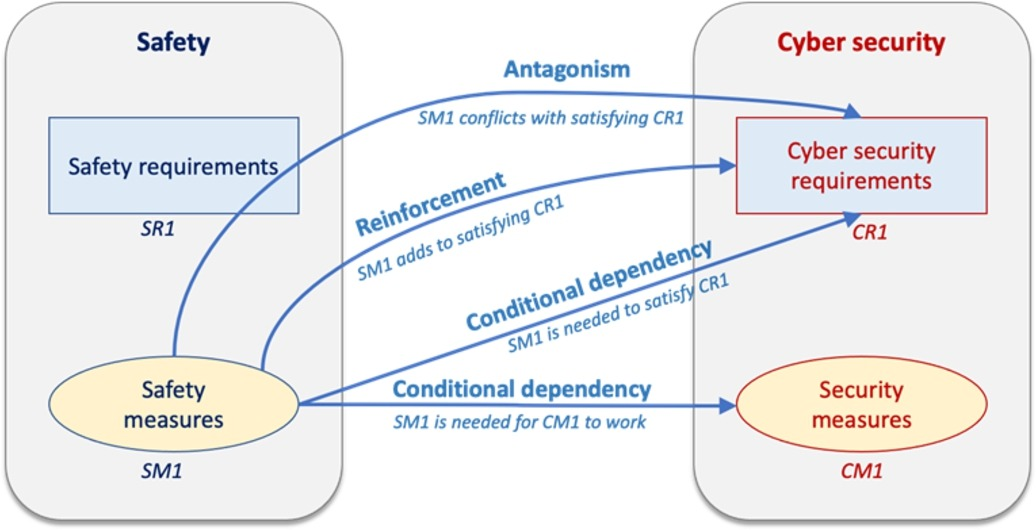
\includegraphics[width=0.5\textwidth]{Image/fig1.jpg}

                &

                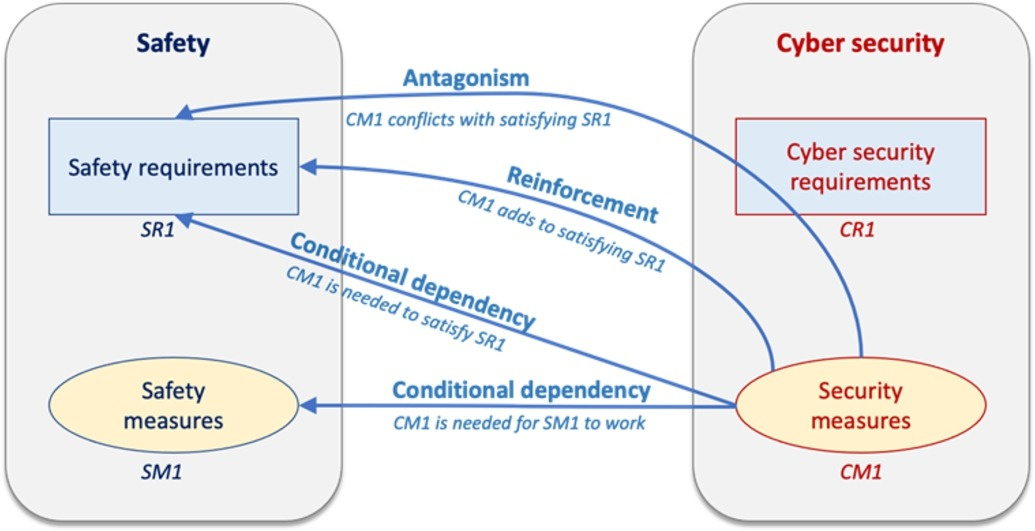
\includegraphics[width=0.5\textwidth]{Image/fig2.jpg} \\

                شکل 1: تاثیر اقدامات ایمنی بر امنیت سایبری

                &

                شکل 2: تاثیر اقدامات امنیت سایبری بر ایمنی
                        
            \end{tabular}

        \end{table}

        علاوه بر وابستگی‌های متقابل بین نیازها و اقدامات ایمنی و امنیت سایبری، ممکن است وابستگی‌هایی بین سطوح خرابی و حمله نیز وجود داشته باشد. به عنوان مثال، یک خرابی ایمنی می‌تواند به فعال‌سازی یک حمله امنیتی کمک کند، یا برعکس. علاوه بر این، یک خرابی ایمنی می‌تواند یک حمله امنیتی را مسدود کند، یا برعکس. بنابراین، دو نوع رابطه جدید می‌توان تعریف کرد: "فعال‌سازی" و "مسدودسازی". ما طبقه‌بندی اولیه وابستگی‌های متقابل ایمنی و امنیت، که توسط Kolb و همکاران (2021) پیشنهاد شده بود، را گسترش داده و روابط "فعال‌سازی" و "مسدودسازی" را اضافه کرده‌ایم، همان‌طور که در شکل 3 نشان داده شده است.

        \begin{table}
            
            \centering
            \begin{tabular}{ c }
                
                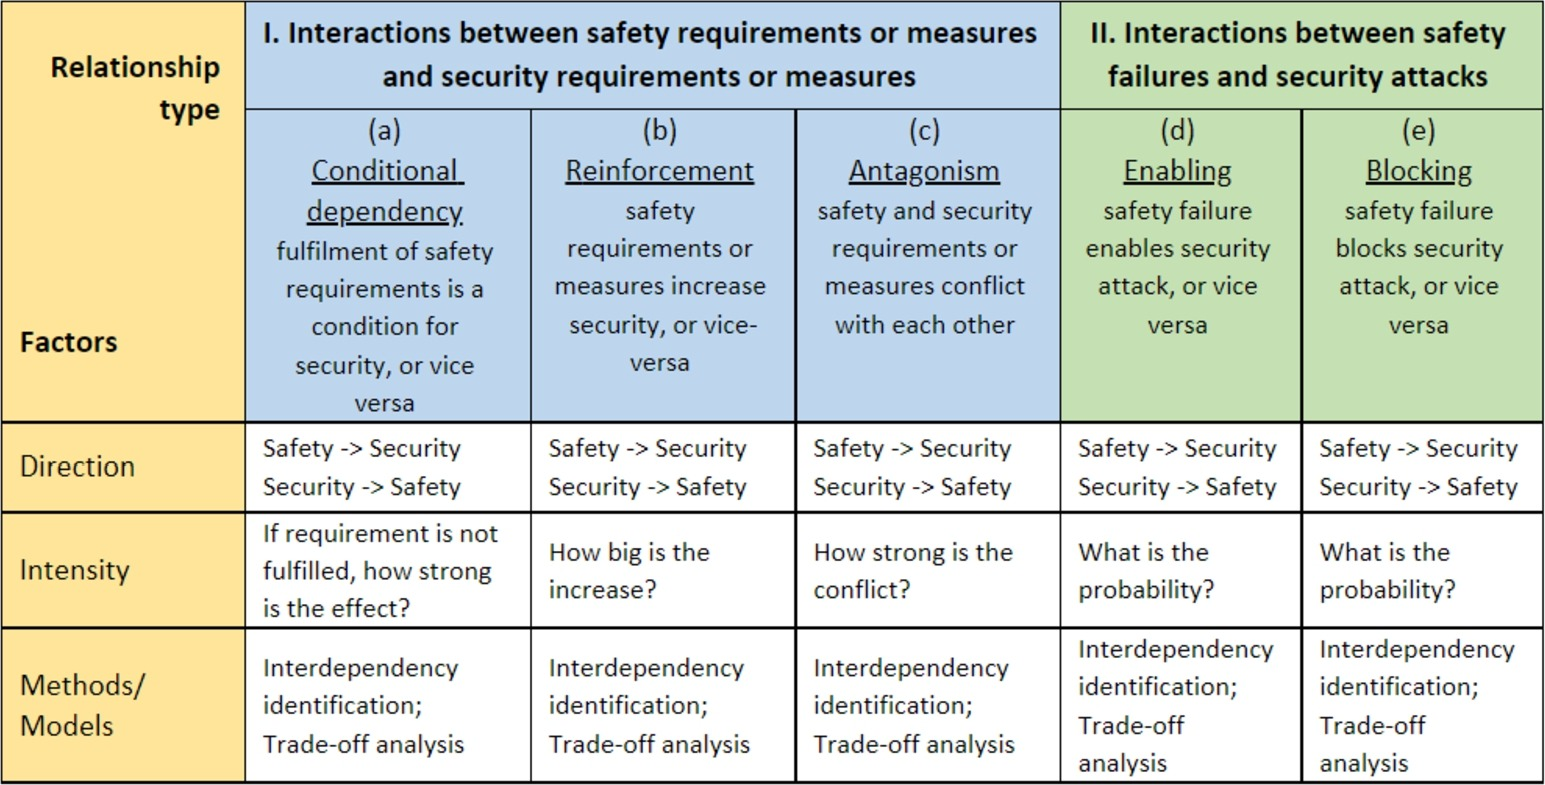
\includegraphics[width=1\textwidth]{Image/fig3.jpg} \\

                شکل 3: امنیت و وابستگی متقابل امنیتی

            \end{tabular}

        \end{table}

        علاوه بر انواع روابط، شکل 3 شامل عوامل مختلفی است که برای تمامی انواع روابط مرتبط هستند، مانند:
        
        \begin{itemize}
            
            \item جهت – دو جهت وجود دارد، یا از ایمنی به امنیت (تأثیر ایمنی بر امنیت) یا برعکس
            
            \item شدت – اندازه‌گیری شدت وابستگی متقابل.

            \item روش‌ها/مدل‌ها – روش‌ها و مدل‌های مختلف برای تسهیل تحلیل وابستگی‌های متقابل

        \end{itemize}

        هدف کار ما ارائه روشی است که به بررسی رابطه بین ایمنی و امنیت سایبری در هر مرحله از چرخه حیات سیستم سایبر فیزیکی (CPS) بپردازد و تعامل بین آن‌ها را برجسته کند.

    \section{مروری بر روش‌شناسی}

        شکل 5 چارچوب روش‌شناسی TOMSAC را نشان می‌دهد که شامل موارد زیر است:
    
        \begin{itemize}
            
            \item مراحل چرخه حیات CPS

            \item تیم‌های درگیر در فرآیند توسعه، مانند تیم‌های طراحی/توسعه، ایمنی و امنیت   سایبری، تأمین‌کنندگان و کاربران؛

            \item نقاط هماهنگی در مراحل مختلف چرخه حیات برای تیم‌ها به منظور هماهنگ کردن محصولات کاری خود و انجام مبادلات، در صورت لزوم.

        \end{itemize}

        تیم‌های متعددی در توسعه CPS درگیر هستند، مانند توسعه‌دهندگان، تیم ایمنی، تیم امنیت سایبری و غیره، که هر کدام استانداردهای خود را دنبال می‌کنند، فرآیندهای مختلفی دارند، محصولات کاری مختلفی توسعه می‌دهند و حتی به زبان‌های مختلفی صحبت می‌کنند یا از اصطلاحات مشابه برای معانی مختلف استفاده می‌کنند، که این امر باعث می‌شود درک کامل یکدیگر و یکپارچه‌سازی نتایج کارشان دشوار باشد. هدف روش‌شناسی TOMSAC فراهم کردن یک چارچوب یکپارچه برای این تیم‌ها است تا ارتباط و هماهنگی کارهایشان را تسهیل کند.

    \section{روش‌شناسی TOMSAC برای حوزه خودرو}

        بخش خودرو، به‌ویژه وسایل نقلیه جاده‌ای خودکار، حوزه اصلی تخصص ما است. بنابراین، ابتدا روش‌شناسی TOMSAC را برای این بخش سفارشی می‌کنیم. مراحل چرخه حیات بر این اساس به فعالیت‌های 26262 ISO ،ISO) 2018) و 21434 ISO/SAE ،ISO/SAE) (2021a تنظیم می‌شوند. 26262 ISO استاندارد ایمنی عملکردی وسایل نقلیه جاده‌ای و 21434 ISO/SAE استاندارد امنیت سایبری است. هر دو استاندارد 26262 ISO و 21434 ISO/SAE نیاز به شناسایی رشته‌های مرتبط و ایجاد و نگهداری کانال‌های ارتباطی بین آن‌ها را دارند. 26262 ISO به‌طور صریح به امنیت سایبری اشاره می‌کند و به‌طور مشابه، 21434 ISO/SAE ایمنی عملکردی را به‌عنوان رشته‌های مرتبط شناسایی می‌کند.

        زیر بخش‌های زیر به توصیف کاربرد روش‌شناسی TOMSAC در مراحل توسعه مفهوم و محصول خودرو می‌پردازند.

        \subsection{مدیریت مبادلات در مرحله مفهوم}

            شکل 4 یک نمای کلی از روش‌شناسی TOMSAC را که در مرحله توسعه مفهوم خودرو به کار گرفته شده است، شامل می‌شود.

            \begin{table}
            
                \centering
                \begin{tabular}{ c }
                    
                    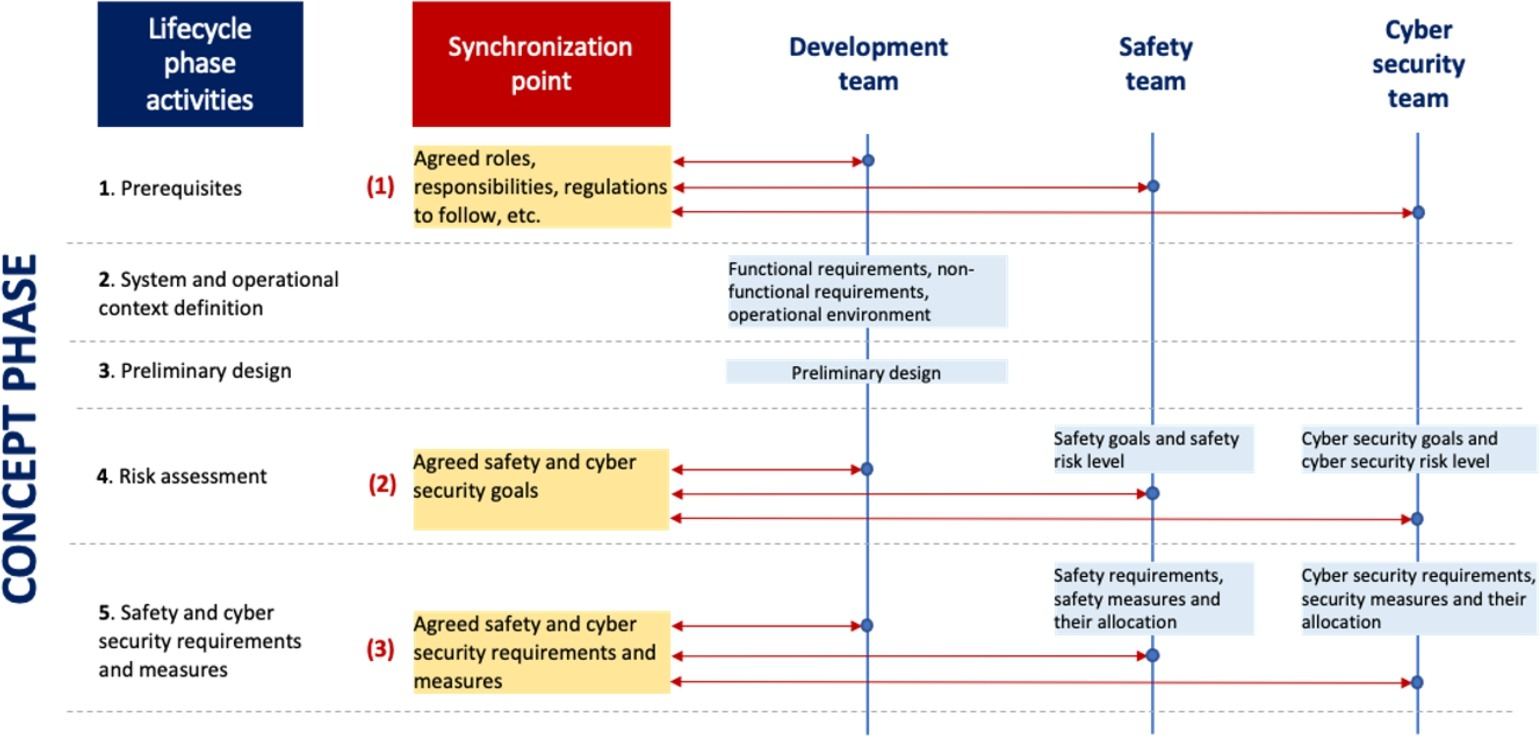
\includegraphics[width=0.6\textwidth]{Image/fig4.jpg} \\
    
                    شکل 4: فعالیت های فاز مفهومی و نقاط هماهنگ سازی بین تیم های توسعه، ایمنی و امنیت سایبری.
    
                \end{tabular}
    
            \end{table}
        
            \begin{table}
            
                \centering
                \begin{tabular}{ c }
                    
                    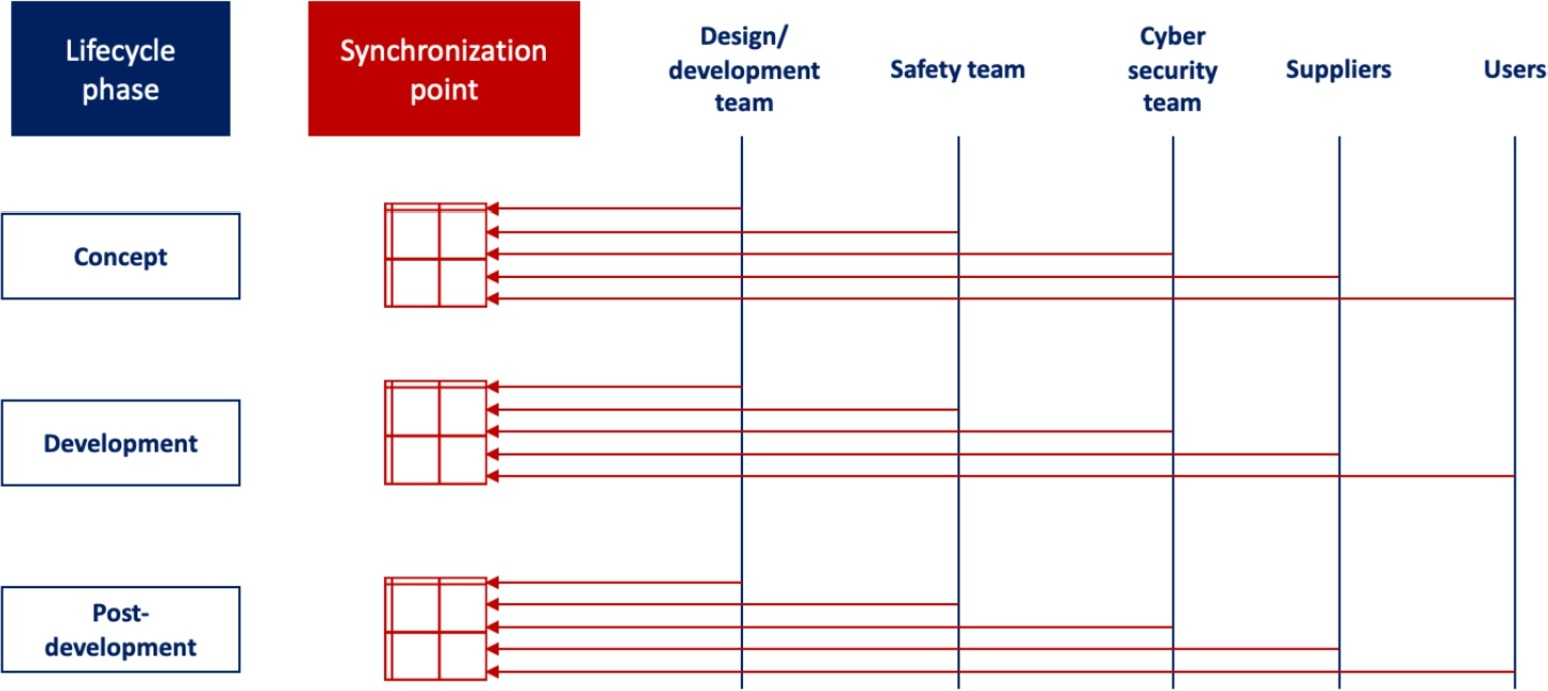
\includegraphics[width=0.6\textwidth]{Image/fig5.jpg} \\
    
                    شکل 5: مراحل چرخه حیات CPS، تیم‌های درگیر و نقاط همگام‌سازی/معادل.
    
                \end{tabular}
    
            \end{table}

            در این مرحله، تولیدکنندگان تجهیزات اصلی خودرو OEM) ها) یا تیم‌های درگیر، مسئولیت‌ها را به اشتراک می‌گذارند و یک مدل مفهومی سیستم توسعه می‌دهند. به عنوان بخشی از مدل مفهومی سیستم، آن‌ها ارزیابی اولیه ریسک را انجام می‌دهند و با توافق بر روی نیازها و اقدامات ایمنی و امنیت سایبری مرتبط به پایان می‌رسانند.

            همان‌طور که در شکل 4 می‌بینیم، سه تیم در این مرحله درگیر هستند: توسعه، ایمنی و امنیت سایبری. ما در این مرحله سه نقطه هم‌زمانی پیشنهاد می‌کنیم تا تیم‌ها محصولات کاری خود را هماهنگ کنند و هرگونه مبادله لازم را انجام دهند.

            \subsubsection{نقطه هم‌زمانی (1): توافق بر نقش‌ها، مسئولیت‌ها و مقررات}

                در این نقطه، باید یک جلسه بین همه تیم‌ها برگزار شود تا در مورد نحوه هماهنگی کارهایشان توافق کنند. توافق می‌تواند شامل تعریف نقش‌ها، مسئولیت‌ها، مقرراتی که آن‌ها دنبال می‌کنند، برنامه‌ها و غیره باشد.

            \subsubsection{نقطه هم‌زمانی (2): توافق بر اهداف ایمنی و امنیت سایبری}

                مفید است که در پایان ارزیابی ریسک یک نقطه هم‌زمانی داشته باشیم، زمانی که اهداف ایمنی و امنیت سایبری (نیازهای سطح بالا) تعریف می‌شوند و سطح ریسک مربوط به آن‌ها تعیین می‌شود. اهداف این نقطه هم‌زمانی دوگانه است:

                \begin{enumerate}
                    
                    \item بررسی اینکه آیا همه دارایی‌های مهم سیستم (از دیدگاه توسعه‌دهندگان) محافظت می‌شوند - یعنی اطمینان حاصل کنیم که تیم‌های ایمنی و امنیت سایبری چیزی را از قلم نینداخته‌اند؛ و

                    \item انجام یک تحلیل اولیه وابستگی متقابل بین ایمنی و امنیت با تحلیل روابط بین اهداف ایمنی و امنیت سایبری.
                    
                \end{enumerate}

                برای دستیابی به هدف اول، می‌توانیم از ماتریس‌های رابطه برای نقشه‌برداری اهداف ایمنی و امنیت سایبری به دارایی‌های سیستم استفاده کنیم، همان‌طور که در شکل 6 نشان داده شده است. در شکل 6، "O" نشان‌دهنده این است که هدف (ردیف) به حفاظت از دارایی (ستون) کمک می‌کند.

                \begin{table}
            
                    \centering
                    \begin{tabular}{ c }
                        
                        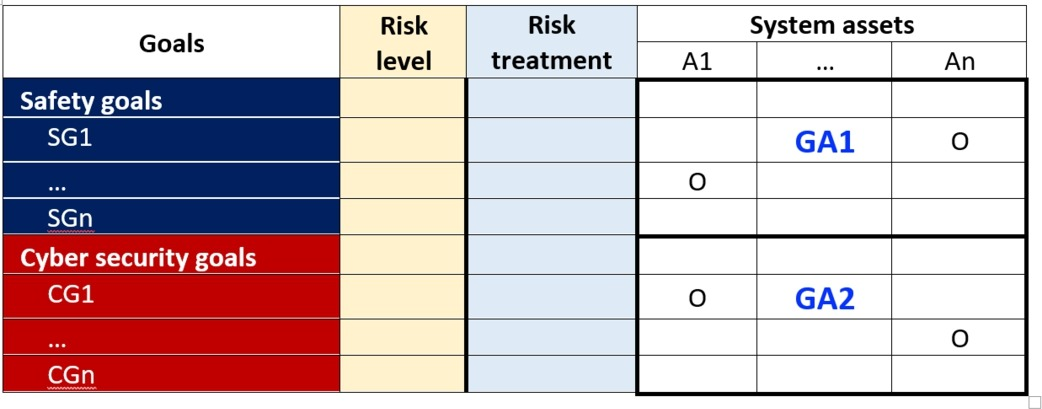
\includegraphics[width=0.5\textwidth]{Image/fig6.jpg} \\
        
                        شکل 6: فعالیت های فاز مفهومی و نقاط هماهنگ سازی بین تیم های توسعه، ایمنی و امنیت سایبری.
        
                    \end{tabular}
        
                \end{table}

                هر سه تیم باید بر اهداف ایمنی و امنیت سایبری، سطوح ریسک و گزینه‌های مدیریت ریسک (کاهش یا اجتناب، اشتراک‌گذاری، حفظ) برای هر دارایی، مطابق با استانداردهای \lr{ISO 26262} و \lr{ISO/SAE 21434} توافق کنند.

                برای دستیابی به هدف دوم، می‌توانیم از ماتریس‌های رابطه GG1 و GG2، که به ترتیب در شکل 7 و شکل 8 نشان داده شده‌اند، استفاده کنیم. GG1 به تحلیل تأثیر اهداف امنیت سایبری بر اهداف ایمنی کمک می‌کند، در حالی که GG2 بر تأثیر اهداف ایمنی بر اهداف امنیت سایبری متمرکز است.

                \begin{table}
            
                    \centering
                    \begin{tabular}{ c }
                        
                        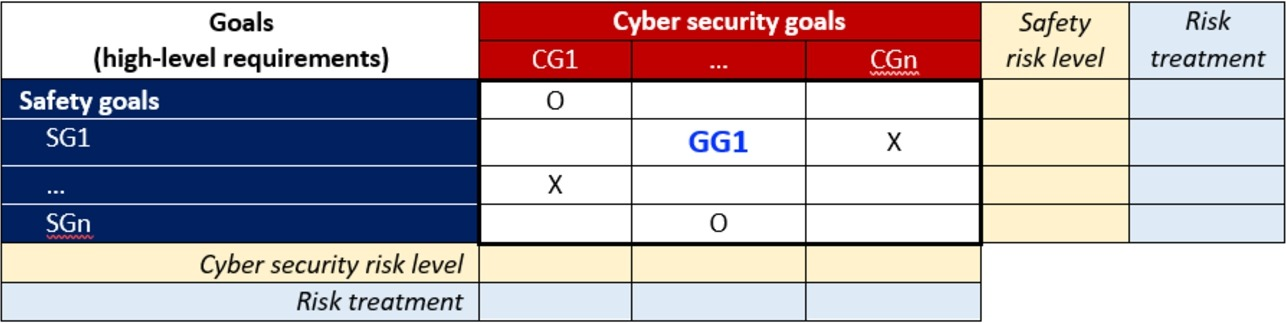
\includegraphics[width=0.5\textwidth]{Image/fig7.jpg} \\
        
                        شکل 7: ماتریس رابطه GG1 برای تحلیل تضاد اهداف امنیت سایبری با اهداف ایمنی.
        
                    \end{tabular}
        
                \end{table}

                \begin{table}
            
                    \centering
                    \begin{tabular}{ c }
                        
                        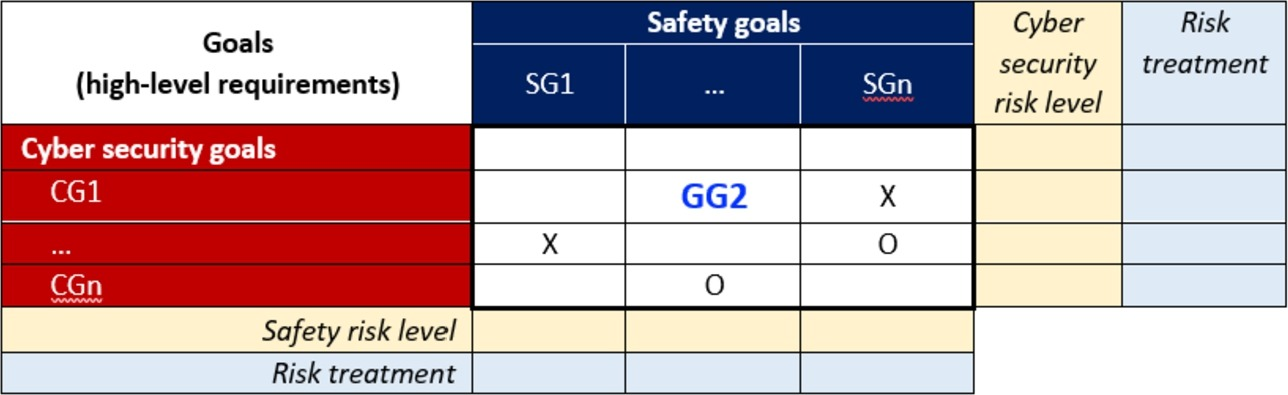
\includegraphics[width=0.5\textwidth]{Image/fig8.jpg} \\
        
                        شکل 8: ماتریس رابطه GG2 برای تحلیل تضاد اهداف ایمنی با اهداف امنیت سایبری.
        
                    \end{tabular}
        
                \end{table}

                در شکل 7، "O" نشان می‌دهد که هدف امنیت سایبری (ستون) به تحقق هدف ایمنی (ردیف) کمک می‌کند، در حالی که "X" به این معنی است که هدف امنیت سایبری (ستون) با هدف ایمنی (ردیف) در تضاد است.

                در همین حال، در شکل 8، "O" نشان می‌دهد که هدف ایمنی (ستون) به تحقق هدف امنیت سایبری (ردیف) کمک می‌کند، در حالی که "X" به این معنی است که هدف ایمنی (ستون) با هدف امنیت سایبری (ردیف) در تضاد است.

                ماتریس‌های GG1 و GG2 همچنین برای توافق بر گزینه‌های مدیریت ریسک برای اهداف ایمنی و امنیت سایبری وابسته به یکدیگر مفید هستند.

            \subsubsection{نقطه هم‌زمانی (3): توافق بر نیازها و اقدامات ایمنی و امنیت سایبری}

                پس از نهایی شدن اهداف ایمنی و امنیت سایبری، نیازهایی با گزینه‌های مدیریت ریسک «کاهش» به نیازهای دقیق‌تری تبدیل می‌شوند – استراتژی‌های مستقل از طراحی برای دستیابی به اهداف. نیازهای ایمنی و امنیت سایبری همچنین به اقدامات ایمنی و امنیتی اختصاص داده می‌شوند که سپس به سیستم‌های وسیله نقلیه یا محیط آن تخصیص می‌یابند.

                در این مرحله، زمانی که اقدامات ایمنی و امنیتی توسط تیم‌های مربوطه تعیین شده‌اند، می‌توانیم شروع به تحلیل وابستگی‌های متقابل احتمالی بین آن‌ها کنیم.

                برای شناسایی و حل تعارضات احتمالی بین اقدامات، می‌توانیم از چارچوب ارزیابی ریسک سایبری (CRAF) Asplund) و همکاران, 2019) استفاده کنیم. روش CRAF شامل موارد زیر است:

                \begin{itemize}
                    
                    \item یک نقشه از پیش تعریف‌شده بین ویژگی‌های امنیت داده و ایمنی (شکل 9 را ببینید)؛

                    \item مجموعه‌ای از جداول، که توسط هر دو تیم ایمنی و امنیتی تکمیل شده‌اند (شکل 10، شکل 11، شکل 12 را ببینید).

                \end{itemize}

                \begin{table}
            
                    \centering
                    \begin{tabular}{ c }
                        
                        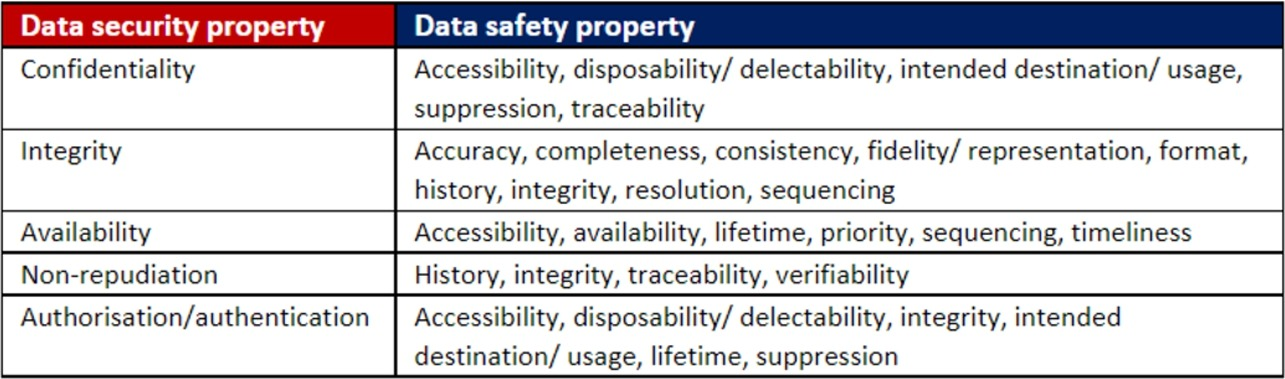
\includegraphics[width=0.6\textwidth]{Image/fig9.jpg} \\
        
                        شکل 9: نقشه‌برداری بین ایمنی داده‌ها و ویژگی‌های امنیتی.
        
                    \end{tabular}
        
                \end{table}

                \begin{table}
            
                    \centering
                    \begin{tabular}{ c }
                        
                        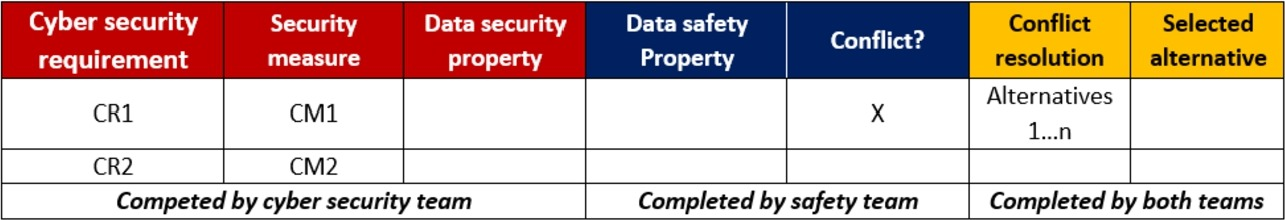
\includegraphics[width=0.6\textwidth]{Image/fig10.jpg} \\
        
                        شکل 10: جدول CRAF برای تجزیه و تحلیل تضاد بین اقدامات امنیتی و ایمنی.
        
                    \end{tabular}
        
                \end{table}

                \begin{table}
            
                    \centering
                    \begin{tabular}{ c }
                        
                        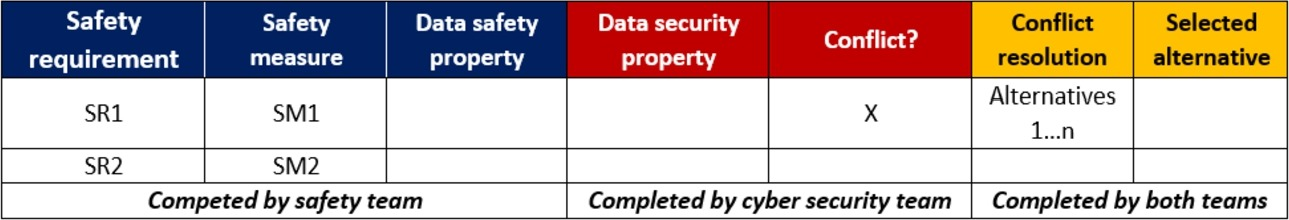
\includegraphics[width=0.6\textwidth]{Image/fig11.jpg} \\
        
                        شکل 11: جدول CRAF برای تجزیه و تحلیل تضاد بین اقدامات ایمنی و امنیت.
        
                    \end{tabular}
        
                \end{table}

                \begin{table}
            
                    \centering
                    \begin{tabular}{ c }
                        
                        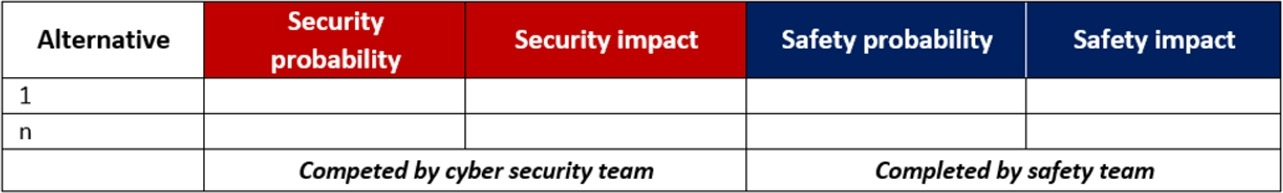
\includegraphics[width=0.6\textwidth]{Image/fig12.jpg} \\
        
                        شکل 12: ارزیابی جایگزین های CRAF
        
                    \end{tabular}
        
                \end{table}

                شکل 10 می‌تواند توسط تیم ایمنی برای تحلیل اینکه آیا نیازها و اقدامات امنیت سایبری با ایمنی در تضاد نیستند، استفاده شود، در حالی که شکل 11 برای بررسی اینکه آیا نیازها و اقدامات ایمنی با امنیت سایبری در تضاد نیستند، استفاده می‌شود.

                اگر تعارضات احتمالی در شکل 10 و شکل 11 شناسایی شوند، هر دو تیم باید سعی کنند تعارضات را با بررسی راه‌حل‌های جایگزین حل کنند. برای ارزیابی راه‌حل‌های جایگزین، می‌توان از شکل 12 استفاده کرد.

                شکل 12 انواع روابط ایمنی و امنیت سایبری را نشان می‌دهد که می‌توان با استفاده از روش CRAF تحلیل کرد. همان‌طور که در شکل 16 می‌بینیم، کار ما رابطه تعارض را در نظر می‌گیرد و مدل‌هایی برای تحلیل وابستگی متقابل و مدیریت مبادلات (ارزیابی راه‌حل‌های جایگزین) شامل می‌شود. گزینه‌ها در کلید به عنوان ورودی‌های ممکن در ماتریس‌های MR1-4 در شکل 14 شامل رضایت، کمک به رضایت و تعارض هستند. این‌ها در شکل 16 ثبت شده‌اند.

                علاوه بر روش CRAF، می‌توانیم از ماتریس‌های رابطه برای کمک به تحلیل انواع دیگر روابط، یعنی وابستگی شرطی و تقویت، استفاده کنیم.شکل 14، یک ماتریس رابطه را نشان می‌دهد که چهار ماتریس کوچکتر، ،MR1-MR4 را برای تحلیل روابط بین نیازها و اقدامات ایمنی/امنیت سایبری یکپارچه می‌کند.

                مراحل تکمیل ماتریس‌های MR1-MR4 به شرح زیر است:

                \begin{enumerate}
                    
                    \item تیم ایمنی ماتریس MR1 را پر می‌کند.

                    \item تیم امنیت سایبری ماتریس MR2 را تکمیل می‌کند.

                    \item تیم امنیت سایبری فهرست اقدامات امنیتی خود را با تیم ایمنی به اشتراک می‌گذارد و تیم ایمنی ماتریس MR3 را تکمیل می‌کند؛

                    \item تیم ایمنی فهرست اقدامات ایمنی را با تیم امنیت سایبری به اشتراک می‌گذارد و تیم امنیت سایبری ماتریس MR4 را تکمیل می‌کند؛

                    \item تیم‌های ایمنی و امنیت سایبری جلسه‌ای برگزار می‌کنند و نتایج ماتریس‌های MR3 و MR4 را برای رسیدن به توافق نهایی در مورد انتخاب اقدامات ایمنی و امنیتی مورد بحث قرار می‌دهند. در صورت بروز تعارض، شکل 12 می‌تواند برای ارزیابی اقدامات جایگزین استفاده شود.

                \end{enumerate}

                اگر داده‌های کمی از اثربخشی اقدامات ایمنی/امنیت سایبری در تحقق نیازها موجود باشد، می‌توان از این داده‌ها در شکل 13 (در سراسر ماتریس‌های (MR1-MR4 استفاده کرد تا نماد "O" که تنها نشان می‌دهد که اقدام به تحقق نیاز کمک می‌کند، اما مشخص نمی‌کند که این اقدام چقدر مؤثر است، جایگزین شود. بنابراین، این ماتریس‌ها می‌توانند برای ثبت اطلاعات "شدت" نیز استفاده شوند.

                \begin{table}
            
                    \centering
                    \begin{tabular}{ c }
                        
                        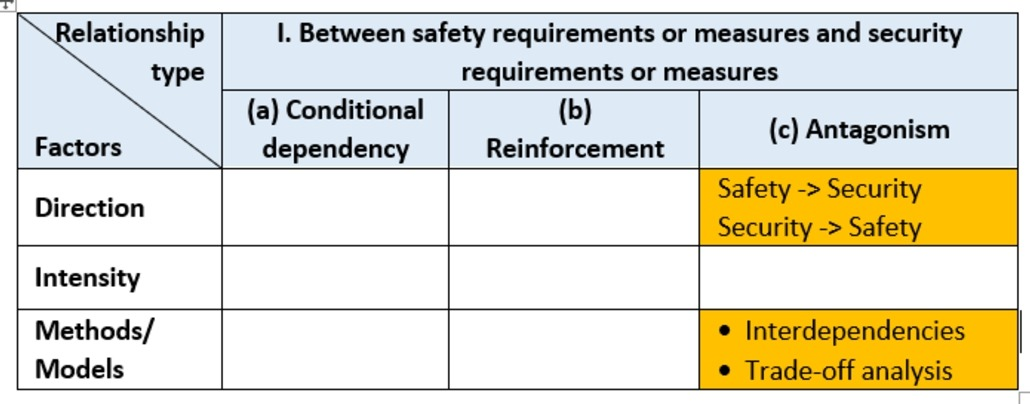
\includegraphics[width=0.6\textwidth]{Image/fig13.jpg} \\
        
                        شکل 13: روابطی که با روش CRAF پرداخته شده است.
        
                    \end{tabular}
        
                \end{table}

                \begin{table}
            
                    \centering
                    \begin{tabular}{ c }
                        
                        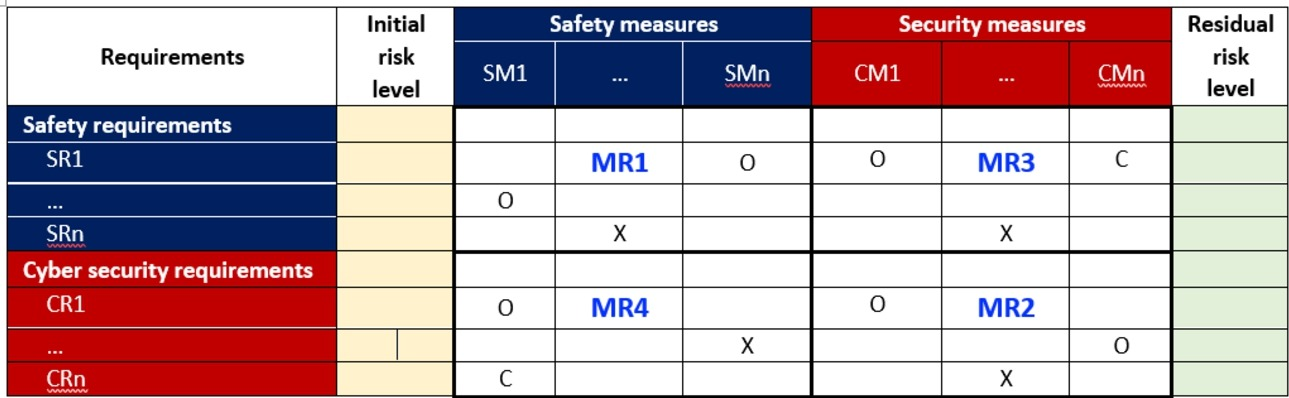
\includegraphics[width=0.6\textwidth]{Image/fig14.jpg} \\
        
                        شکل 14: ماتریس‌های رابطه MR1–MR4 برای وابستگی‌های متقابل بین اقدامات و نیازها.\\
                        
                        O – اقدام (ستون) به تحقق نیاز (ردیف) کمک می‌کند؛\\
                        
                        C – داشتن اقدام (ستون) شرطی برای تحقق نیاز است؛\\
                        
                        X – اقدام (ستون) ممکن است نیاز (ردیف) را نقض کند.
        
                    \end{tabular}
        
                \end{table}

                شکل 16 انواع روابط ایمنی و امنیت سایبری مورد نظر در ماتریس‌های پیشنهادی تاکنون را خلاصه می‌کند.

                پس از نهایی شدن انتخاب اقدامات ایمنی و امنیت سایبری توسط تیم‌های ایمنی و امنیت سایبری، آن‌ها باید با تیم توسعه در مورد تخصیص این اقدامات به سیستم‌های سطح وسیله نقلیه که آیتم (عملکرد سطح وسیله نقلیه) را اجرا می‌کنند یا به محیط توافق کنند. برای تسهیل این فرآیند، می‌توان از ماتریس‌های رابطه ME1-ME2، که اقدامات را به سیستم‌های وسیله نقلیه یا محیط نگاشت می‌کنند، استفاده کرد، همان‌طور که در شکل 17 نشان داده شده است.

                این ماتریس‌ها به ویژه برای یکپارچه‌سازی نتایج تحلیل تهدیدات چندین آیتم مفید هستند، زیرا هر آیتم به طور مستقل تحلیل می‌شود، بنابراین نیازهای ایمنی و امنیت سایبری به طور مستقل مشخص و اقدامات انتخاب می‌شوند.

            \subsubsection{خلاصه‌ای از ماتریس‌های استفاده شده در مرحله مفهومی}

                شکل 15 و شکل 18 خلاصه‌ای از ماتریس‌های استفاده شده در مرحله مفهومی را ارائه می‌دهند. در مجموع 10 ماتریس وجود دارد: چهار ماتریس در سطح هدف و شش ماتریس در سطح نیازمندی‌ها ساخته شده‌اند.

                \begin{table}
            
                    \centering
                    \begin{tabular}{ c }
                        
                        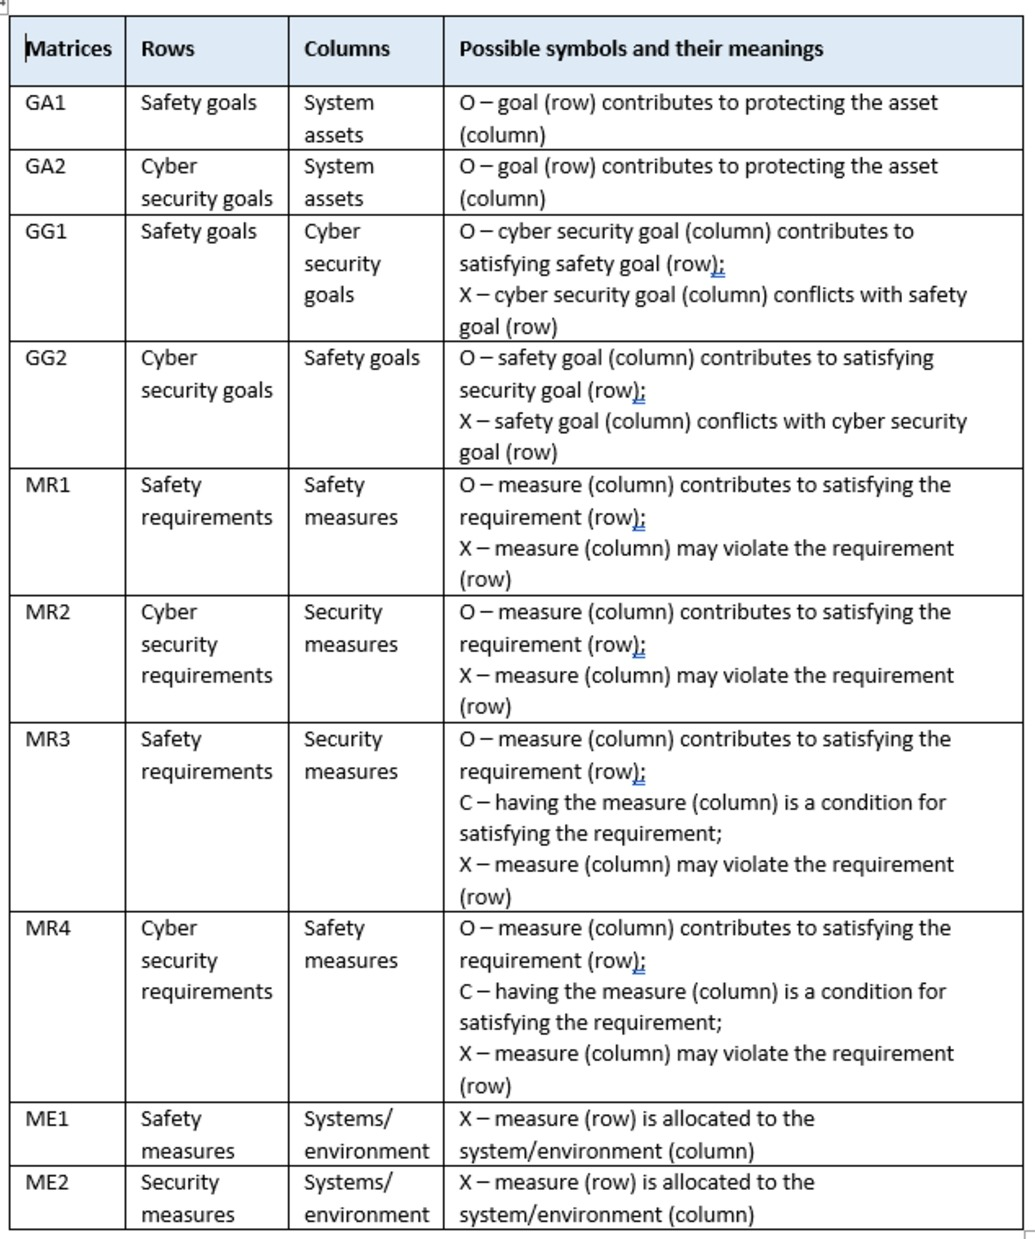
\includegraphics[width=0.8\textwidth]{Image/fig15.jpg} \\
        
                        شکل 15: شرح 10 ماتریس مورد استفاده در فاز مفهومی.

                    \end{tabular}
        
                \end{table}

                \begin{table}
            
                    \centering
                    \begin{tabular}{ c }
                        
                        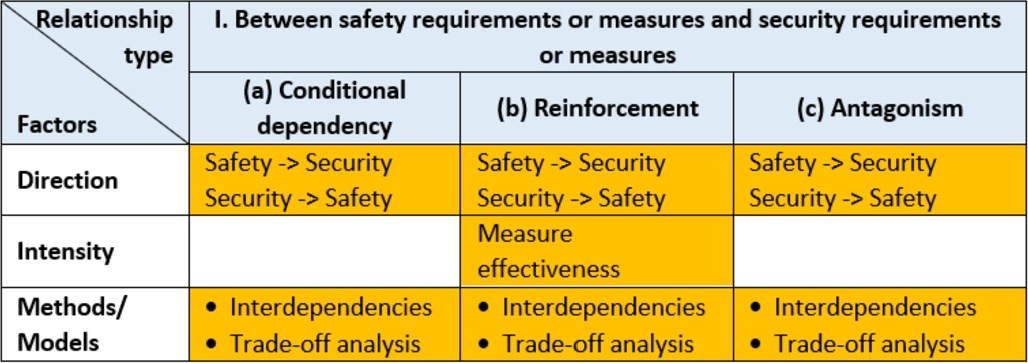
\includegraphics[width=0.6\textwidth]{Image/fig16.jpg} \\
        
                        شکل 16: روابط پرداخته شده توسط ماتریس های GG1-GG2 و MR1-MR4

                    \end{tabular}
        
                \end{table}

                \begin{table}
            
                    \centering
                    \begin{tabular}{ c }
                        
                        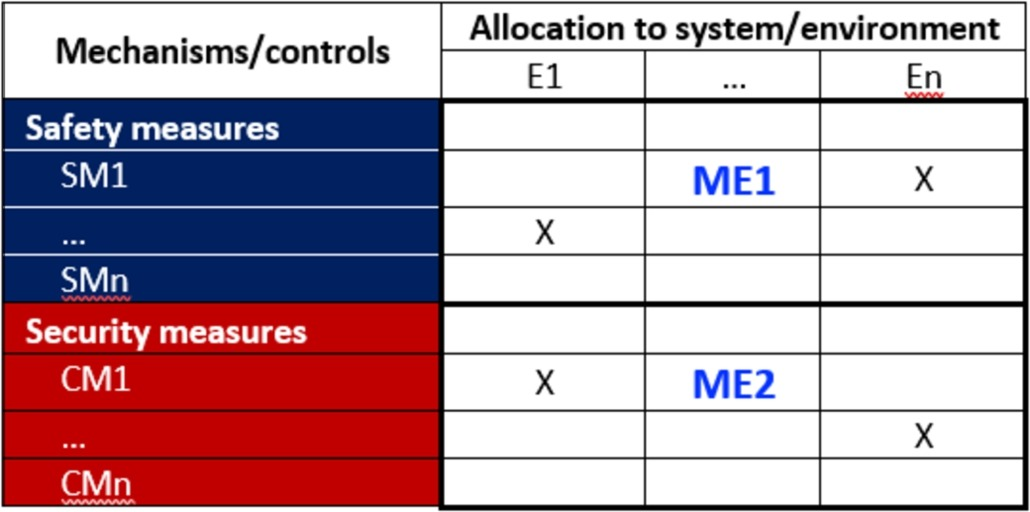
\includegraphics[width=0.6\textwidth]{Image/fig17.jpg} \\
        
                        شکل 17: ماتریس های رابطه ME1 و ME2 برای تخصیص اقدامات ایمنی و امنیتی به سیستم های خودرو/محیط\\
                        X - اندازه گیری (ردیف) به آیتم/محیط (ستون) اختصاص داده می شود

                    \end{tabular}
        
                \end{table}

                \begin{table}
            
                    \centering
                    \begin{tabular}{ c }
                        
                        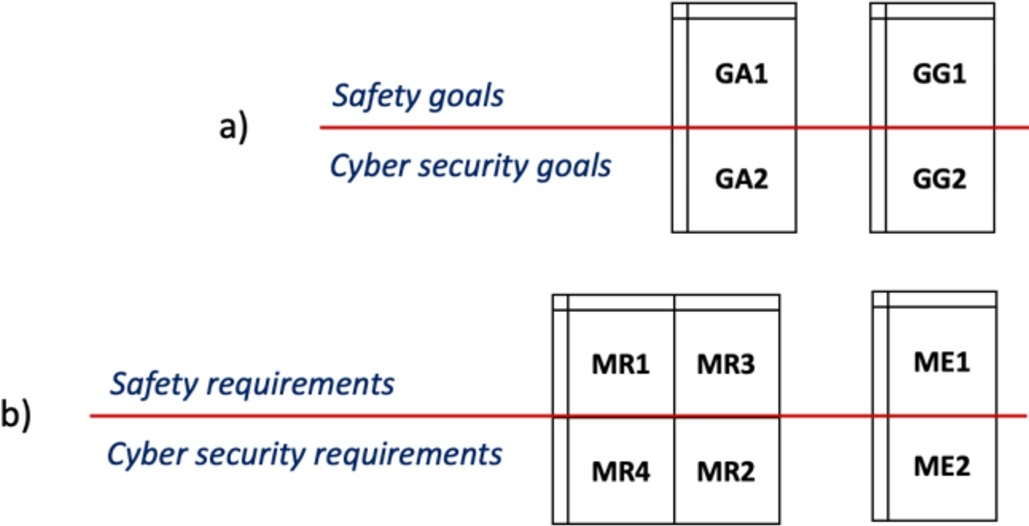
\includegraphics[width=0.6\textwidth]{Image/fig18.jpg} \\
        
                        شکل 18: خلاصه ماتریس فاز مفهومی در: الف) سطح هدف. ب) سطح نیاز.

                    \end{tabular}
        
                \end{table}

        \subsection{مدیریت مبادلات در مرحله توسعه محصول}

            در مرحله توسعه محصول، ما چهار نقطه همگام‌سازی داریم، همان‌طور که در شکل 19 نشان داده شده است.

            \begin{table}
            
                \centering
                \begin{tabular}{ c }
                    
                    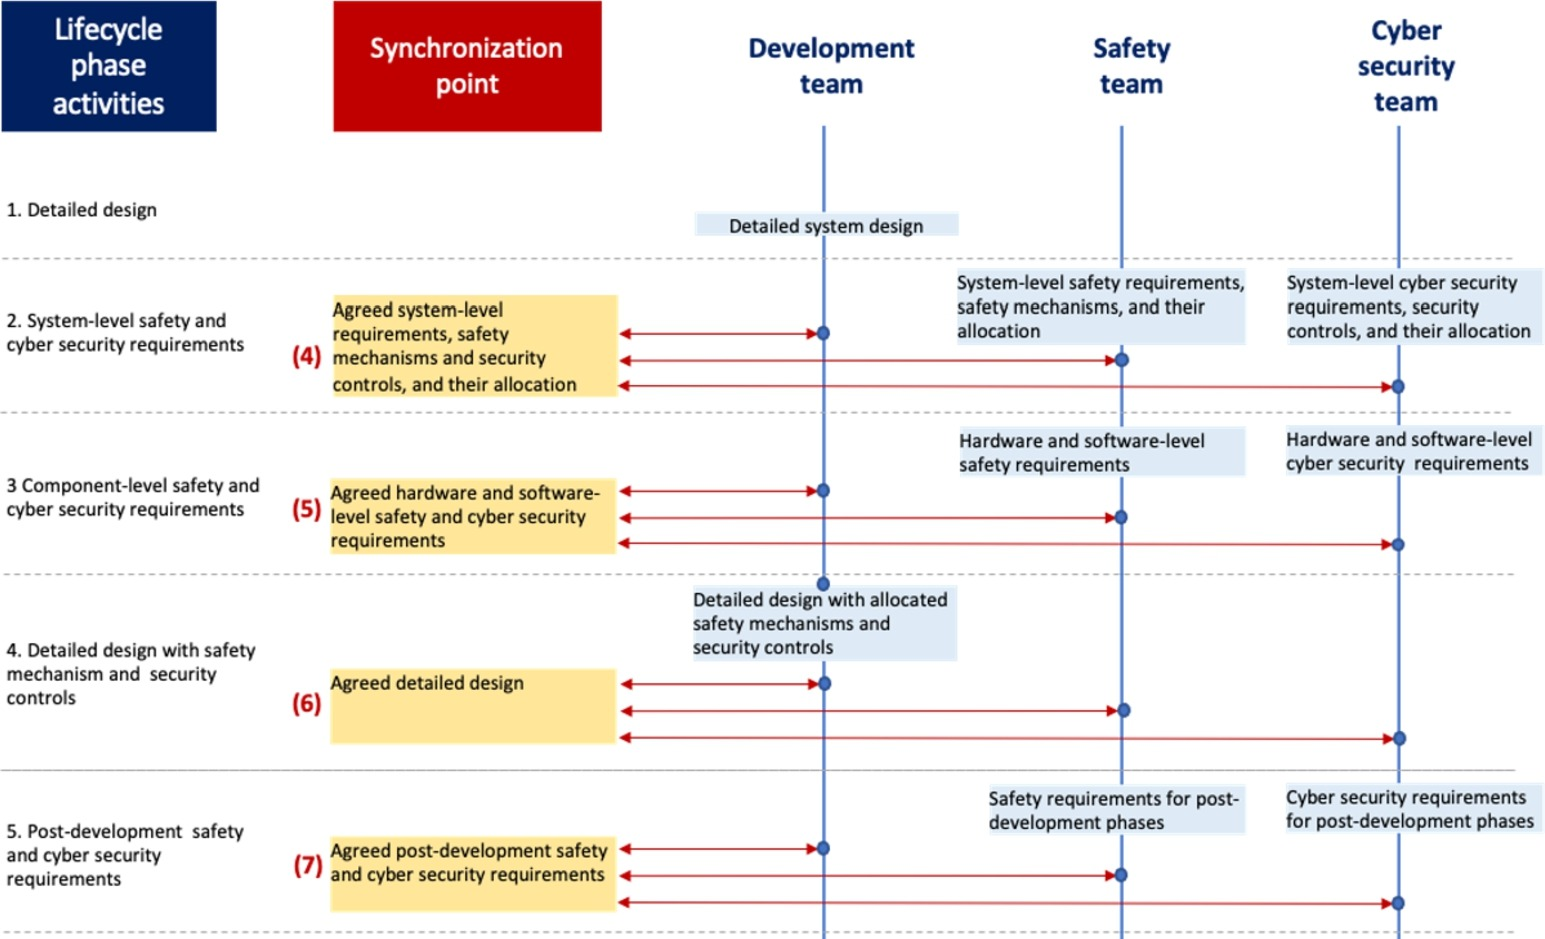
\includegraphics[width=0.8\textwidth]{Image/fig19.jpg} \\
    
                    شکل 19: فعالیت های مرحله توسعه محصول و نقاط هماهنگ سازی بین تیم های توسعه، ایمنی و امنیت سایبری.

                \end{tabular}
    
            \end{table}

            \subsubsection{نقطه همگام‌سازی (4): توافق بر روی نیازمندی‌های سطح سیستم، مکانیزم‌های ایمنی و کنترل‌های امنیتی، و تخصیص آن‌ها}

                پس از توسعه یک طراحی سیستم دقیق توسط تیم توسعه، تیم‌های ایمنی و امنیت سایبری می‌توانند نیازمندی‌های ایمنی و امنیت سایبری سطح مفهومی را به نیازمندی‌های دقیق‌تر سطح سیستم تبدیل کنند. علاوه بر این، اقدامات ایمنی و امنیتی سطح مفهومی به مکانیزم‌های فنی ایمنی و کنترل‌های امنیتی تبدیل می‌شوند که به عناصر مربوطه سیستم اختصاص داده می‌شوند. در این مرحله می‌توان از چندین ماتریس رابطه برای کمک به تیم‌ها در شناسایی وابستگی‌های متقابل و انجام مبادلات در صورت نیاز استفاده کرد.

                ابتدا، ماتریس‌های MR5-MR8 می‌توانند ساخته شوند، همان‌طور که در شکل 20 نشان داده شده است. این ماتریس‌ها نسخه‌های دقیق‌تر MR1-MR4 هستند که در مرحله مفهومی توسعه یافته‌اند.

                \begin{table}
            
                    \centering
                    \begin{tabular}{ c }
                        
                        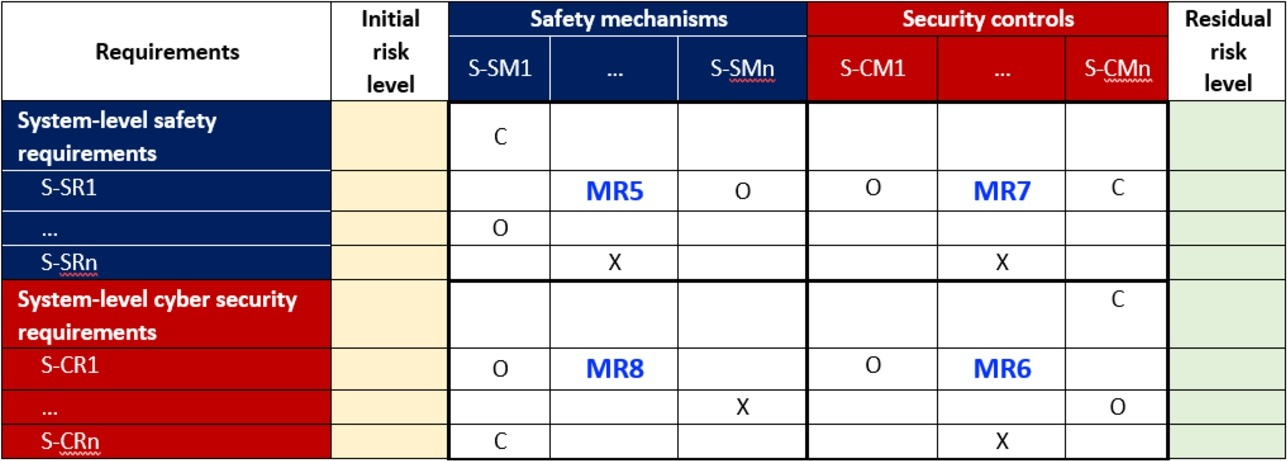
\includegraphics[width=0.6\textwidth]{Image/fig20.jpg} \\
        
                        شکل 20: ماتریس‌های رابطه‌ای MR5–MR8 برای تحلیل وابستگی‌های متقابل بین مکانیزم‌ها و نیازمندی‌ها.\\
                        
                        O – مکانیزم/کنترل (ستون) به تحقق نیازمندی (ردیف) کمک می‌کند؛\\
                        
                        C – داشتن مکانیزم/کنترل (ستون) شرط لازم برای تحقق نیازمندی است؛\\
                        
                        X – مکانیزم/کنترل (ستون) ممکن است نیازمندی (ردیف) را نقض کند.
    
                    \end{tabular}
        
                \end{table}

                مراحل زیر برای تکمیل ماتریس‌های MR5-MR8 است:

                \begin{enumerate}
                    
                    \item تیم ایمنی ماتریس MR5 را تکمیل می‌کند.

                    \item تیم امنیت سایبری ماتریس MR6 را تکمیل می‌کند.

                    \item تیم امنیت سایبری فهرست کنترل‌های امنیتی خود را با تیم ایمنی به اشتراک می‌گذارد و تیم ایمنی ماتریس MR7 را تکمیل می‌کند؛

                    \item تیم ایمنی فهرست مکانیزم‌های ایمنی خود را با تیم امنیت سایبری به اشتراک می‌گذارد تا ماتریس MR8 را تکمیل کنند؛

                    \item تیم‌های ایمنی و امنیت سایبری دیدار می‌کنند و نتایج ماتریس‌های MR5-MR8 را برای رسیدن به توافق نهایی در مورد انتخاب اقدامات ایمنی و امنیتی بحث می‌کنند. در صورت وجود تضادها، تیم‌ها باید مبادلاتی انجام دهند تا تضادها را حذف کنند و در عین حال سطح ریسک باقی‌مانده قابل قبول را حفظ کنند.

                \end{enumerate}

                پس از نهایی شدن انتخاب مکانیزم‌های ایمنی و کنترل‌های امنیتی توسط تیم‌های ایمنی و امنیت سایبری، باید با تیم توسعه درباره تخصیص اقدامات به عناصر سیستم به توافق برسند. برای تسهیل این فرآیند، ماتریس‌های رابطه‌ای ME3-ME4، که مکانیزم‌های ایمنی و کنترل‌های امنیتی را به عناصر سیستم نقشه‌برداری می‌کنند، در شکل 21 نشان داده شده‌اند.

                \begin{table}
            
                    \centering
                    \begin{tabular}{ c }
                        
                        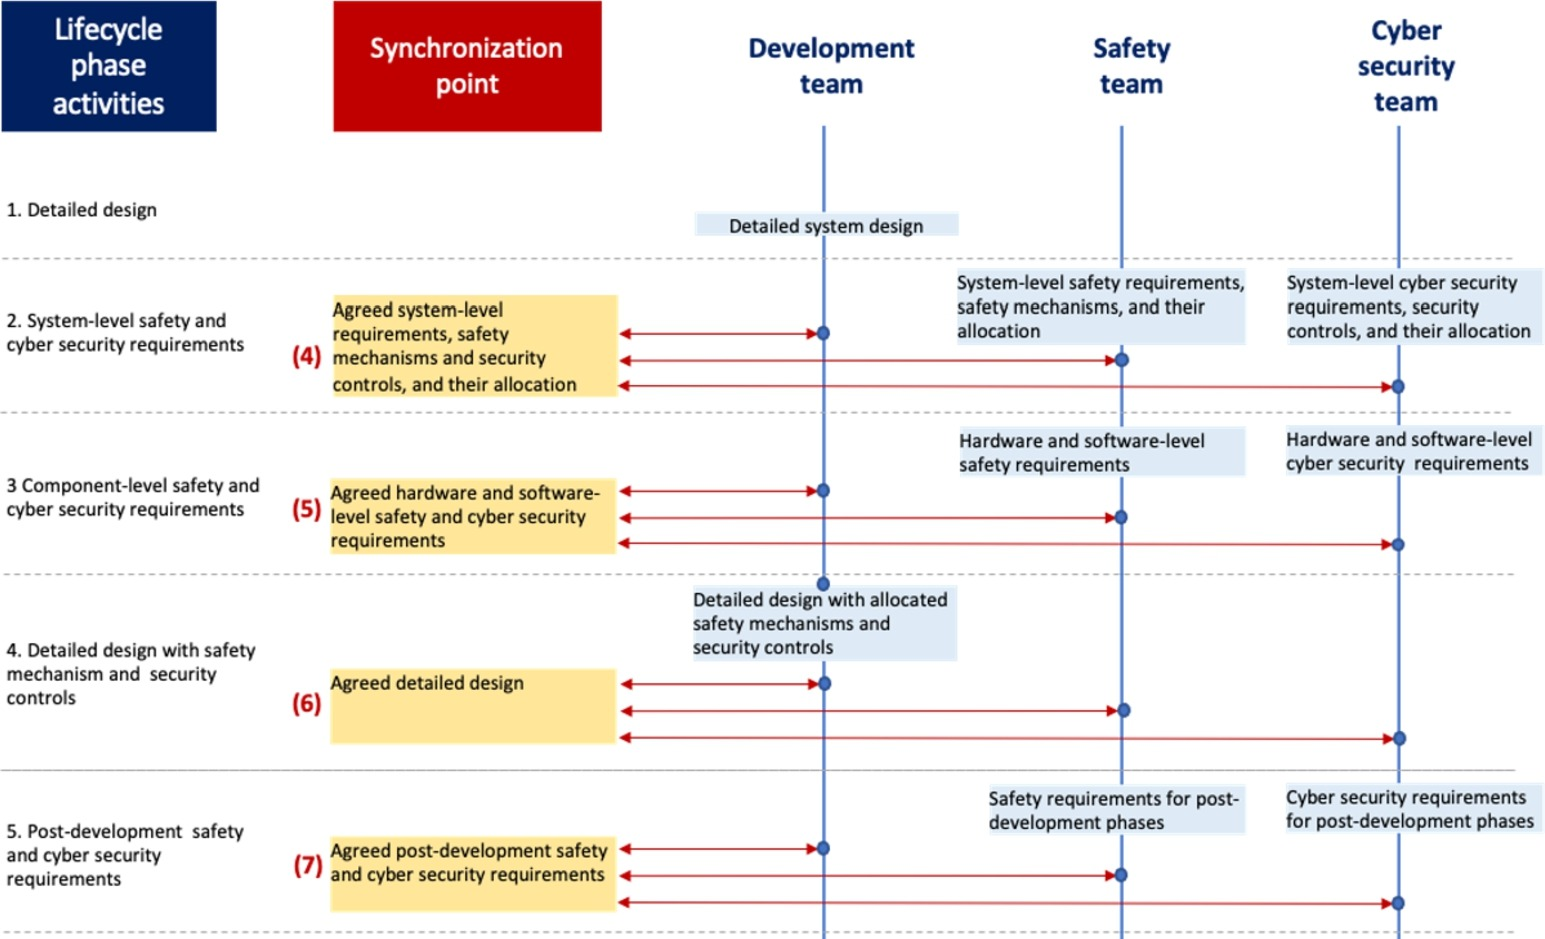
\includegraphics[width=0.8\textwidth]{Image/fig19.jpg} \\
        
                        شکل 21: ماتریس‌های رابطه ME3 و ME4 برای تخصیص مکانیسم‌های ایمنی و کنترل‌های امنیتی به عناصر سیستم.\\
                        
                        X – مکانیزم/کنترل (ردیف) به عنصر سیستم (ستون) اختصاص داده شده است.
    
                    \end{tabular}
        
                \end{table}

            \subsubsection{نقطه هماهنگی (۵): توافق بر روی الزامات ایمنی و امنیت سایبری در سطح سخت‌افزار و نرم‌افزار}

                در این مرحله، الزامات امنیت سایبری در سطح سیستم به الزامات امنیت سایبری در سطح سخت‌افزار و نرم‌افزار تصحیح و مشخص می‌شوند.

                این نقطه هماهنگی به شناسایی وابستگی‌های ممکن بین الزامات ایمنی و امنیت سایبری برای اجزای سخت‌افزاری و نرم‌افزاری مشابه می‌پردازد. چهار ماتریس RE1 تا RE4 می‌توانند برای این منظور استفاده شوند، همانطور که در شکل ۲۲ نشان داده شده است. علاوه بر این، این ماتریس‌ها برای تعریف الزامات عملکردی اجزای نرم‌افزاری/سخت‌افزاری نیز مفید هستند.

                \begin{table}
            
                    \centering
                    \begin{tabular}{ c }
                        
                        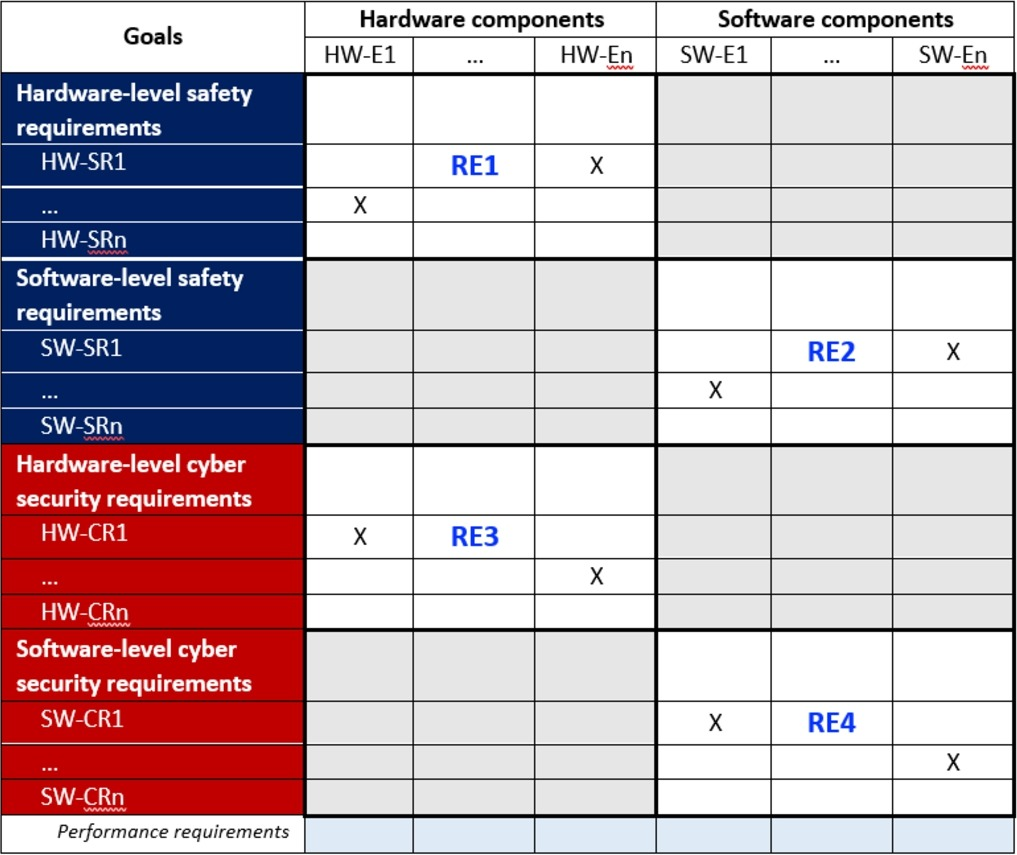
\includegraphics[width=0.8\textwidth]{Image/fig22.jpg} \\
        
                        شکل 22: ماتریس‌های ارتباطی RE1-RE4 برای تخصیص الزامات سخت‌افزاری و نرم‌افزاری\\
                        
                        در سطح سخت‌افزار به قطعات سخت‌افزاری و نرم‌افزاری.\\

                        X - نیاز (ردیف) به جز سخت افزاری یا نرم افزاری (ستون) اختصاص داده می شود.
    
                    \end{tabular}
        
                \end{table}

            \subsubsection{نقطه هماهنگی (۶): توافق بر روی طراحی دقیق}

                در این مرحله، مکانیزم‌های ایمنی و کنترل‌های امنیت سایبری توسط تیم توسعه به طراحی دقیق سیستم اضافه می‌شوند، که سپس نیاز است توسط هر سه تیم بررسی شوند.

            \subsubsection{نقطه هماهنگی (۷): توافق بر روی الزامات ایمنی و امنیت سایبری پس از توسعه}

                در پایان مرحله توسعه محصول، الزامات ایمنی و امنیت سایبری برای مرحله پس از توسعه باید تعریف شوند. این مراحل شامل تولید، عملیات و نگهداری، و از رده خارج کردن هستند. یک ماتریس رابطه‌ای می‌تواند برای هر مرحله استفاده شود، همانطور که در شکل ۲۳ نشان داده شده است. در مجموع، شش ماتریس تعریف شده‌اند، RA1 تا .RA6

                \begin{table}
            
                    \centering
                    \begin{tabular}{ c }
                        
                        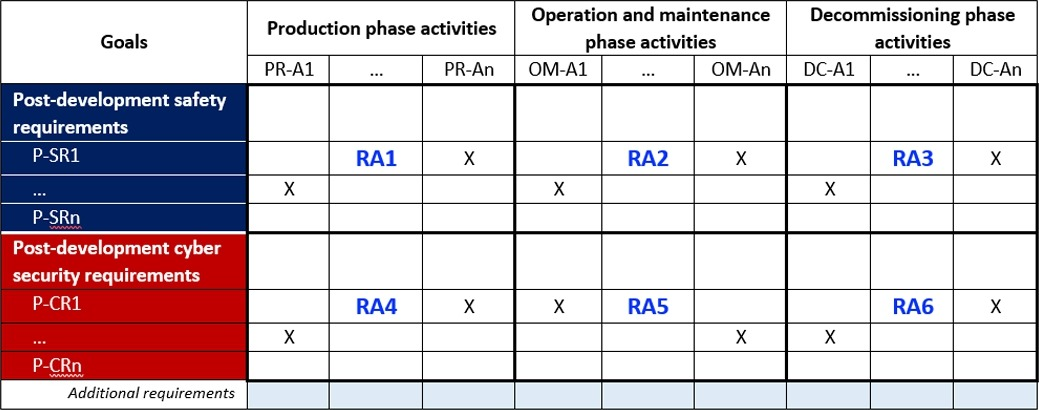
\includegraphics[width=0.6\textwidth]{Image/fig23.jpg} \\
        
                        شکل 23: ماتریس های رابطه RA1-RA6 برای تخصیص الزامات ایمنی و امنیت سایبری به فعالیت های مرحله پس از توسعه.\\

                        X - نیاز (ردیف) به یک فعالیت (ستون) اختصاص داده می شود.
                        
                    \end{tabular}
        
                \end{table}

                الزامات اضافی برای فعالیت‌های فاز پس از توسعه، به منظور تسهیل پیاده‌سازی الزامات ایمنی و امنیت سایبری پس از توسعه، می‌توانند در انتهای شکل ۲۳ تعریف و اضافه شوند.

            \subsubsection{خلاصه‌ای از ماتریس‌های مورد استفاده در مرحله توسعه محصول}

                شکل ۲۳ و شکل ۲۴ شامل یک خلاصه از ماتریس‌های مورد استفاده در مرحله توسعه محصول هستند.

                \begin{table}
            
                    \centering
                    \begin{tabular}{ c }
                        
                        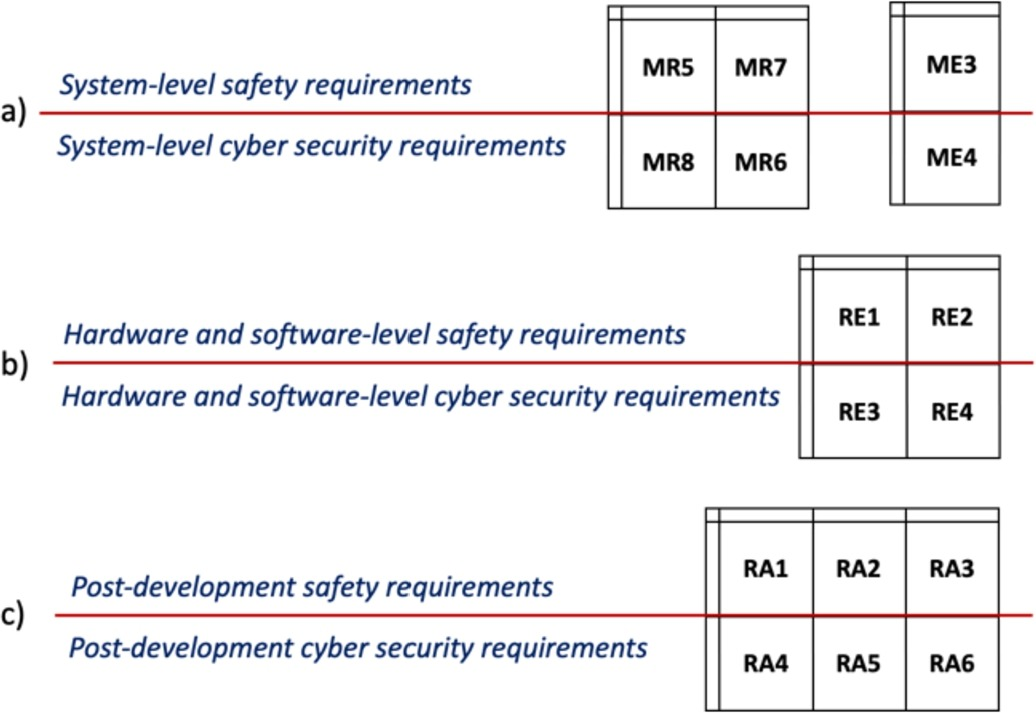
\includegraphics[width=0.6\textwidth]{Image/fig24.jpg} \\

                        شکل 24: خلاصه ای از ماتریس های فاز توسعه محصول در:\\
                        
                        الف) سطح نیاز در سطح سیستم.
                        
                        ب) سطح نیاز سخت افزار و نرم افزار؛
                        
                        ج) سطح نیاز پس از توسعه.

                    \end{tabular}
        
                \end{table}

                در مجموع، شانزده ماتریس برای این فاز تعریف شده است: شش ماتریس برای تحلیل تعاملات در سطح الزامات سیستم؛ چهار ماتریس برای تحلیل در سطح الزامات سخت‌افزاری و نرم‌افزاری؛ و شش ماتریس برای تحلیل در سطح الزامات پس از توسعه.

\end{document}